\chapter{Euler's Method}

How do computers approximate the solution to a differential equation that 
cannot be explicitly solved? Let's consider the differential equation 
$$\frac{dy}{dx} = x + y \text{ with initial condition } y(0) = 1$$.

This means the solution passes through the point (0, 1). Additionally, the 
slope of the solution is $\frac{dy}{dx} = 0 + 1 = 1$ at that point. This means 
we can approximate the solution with the linear function $L(x) = x + 1$ (see 
figure \ref{fig:euler1}). As you can see, near $(0,1)$ the approximation is 
good, but as $x$ increases, the divergence between the actual solution and the 
approximation grows. 

\begin{figure}[htbp]
\centering
\begin{tikzpicture}
    \begin{axis}[xmin = -0.1, xmax = 1.2, xtick = {1}, ymin = -0.3, ymax = 5, 
    ytick = {1}, axis lines = center, xlabel = $x$, ylabel = $y$]
    \addplot[red, domain = 0:1]{-1*x + 2*e^x - 1};
    \addplot[blue, thick, domain = 0:1]{x + 1};
    \node[red] at (0.5, 3) {solution curve};
    \node[blue] at (0.75, 0.9) {$L(x)$};
    \end{axis}
\end{tikzpicture}
\caption{A first Euler approximation}
\label{fig:euler1}
\end{figure}

How can we make a better approximation? Suppose we stop the first 
approximation at $x = 1.5$, re-evaluate $\frac{dy}{dx}$, and use that to make 
a second linear approximation. When $x = 0.5$, $L(x) = 0.5 + 1 = 1.5$. Taking 
the point $(0.5, 1.5)$, then $\frac{dy}{dx} = 0.5 + 1.5 = 2$. We can then 
write a second linear approximation, $L_2(x) = 2(x - 0.5) + 1.5 = 2x - 1 + 1.5 
= 2x + 0.5$. As you can see (figure \ref{fig:euler2}), this new approximation 
is closer than our first approximation. We call this an approximation with a 
step size of 0.5.

\begin{figure}[htbp]
\centering
\begin{tikzpicture}
    \begin{axis}[xmin = -0.1, xmax = 1.2, xtick = {1}, ymin = -0.3, ymax = 5, 
    ytick = {1}, axis lines = center, xlabel = $x$, ylabel = $y$]
    \addplot[red, domain = 0:1]{-1*x + 2*e^x - 1};
    \addplot[blue, thick, domain = 0:0.5]{x + 1};
    \addplot[blue, thick, domain = 0.5:1]{2*x + 0.5};
    \draw[black, dashed](0.5, 0) -- (0.5, 1.5);
    \node[red] at (0.5, 3) {solution curve};
    \node[blue] at (0.25, 0.9) {$L(x)$};
    \node[blue] at (0.75, 1) {$L_2(x)$};
    \end{axis}
\end{tikzpicture}
\caption{An Euler approximation with step size 0.5}
\label{fig:euler2}
\end{figure}

We can improve this further by taking a step size of 0.25 (see figure 
\ref{fig:euler3}). As the step size decreases and the step number increases, 
the approximation gets closer and closer to the true solution. 

\begin{figure}[htbp]
\centering
\begin{tikzpicture}
    \begin{axis}[xmin = -0.1, xmax = 1.2, xtick = {1}, ymin = -0.3, ymax = 5, 
    ytick = {1}, axis lines = center, xlabel = $x$, ylabel = $y$]
    \addplot[red, domain = 0:1]{-1*x + 2*e^x - 1};
    \addplot[blue, thick, domain = 0:0.25]{x + 1};
    \addplot[mark=*, blue](0.25, 1.25);
    \addplot[blue, thick, domain = 0.25:0.5]{1.5*(x - 0.25) + 1.25};
    \addplot[mark=*, blue](0.5, 1.625);
    \addplot[blue, thick, domain = 0.5:0.75]{2.125*(x - 0.5) + 1.625};
    \addplot[mark=*, blue](0.75, 2.15625);
    \addplot[blue, thick, domain = 0.75:1]{2.90625*(x - 0.75) + 2.15625};
    \addplot[mark=*, blue](1, 2.88281);
    \end{axis}
\end{tikzpicture}
\caption{An Euler approximation with step size 0.25}
\label{fig:euler3}
\end{figure}

In general, Euler's method is a numerical process similar to sketching a 
solution on a slope field. One begins at the given initial value, proceeds for 
a short step in the direction indicated by the slope field. You adjust the 
slope of your approximation based on the value of the slope field at the end 
of each step. 

For a first-order differential equation, let $\frac{dy}{dx} = F(x, y)$ and 
$y(x_0) = y_0$. If we have step size $h$, then our successive $x$-values are 
$x_1 = x_0 + h$, $x_2 = x_1 + h$, etc. The differential equation tells us that 
the slope at $x_0$ is $F(x_0, y_0)$. So, $y_1 = y_0 + hF(x_0, y_0)$ (see 
figure \ref{fig:eulervis}). 

\begin{figure}[htbp]
\centering
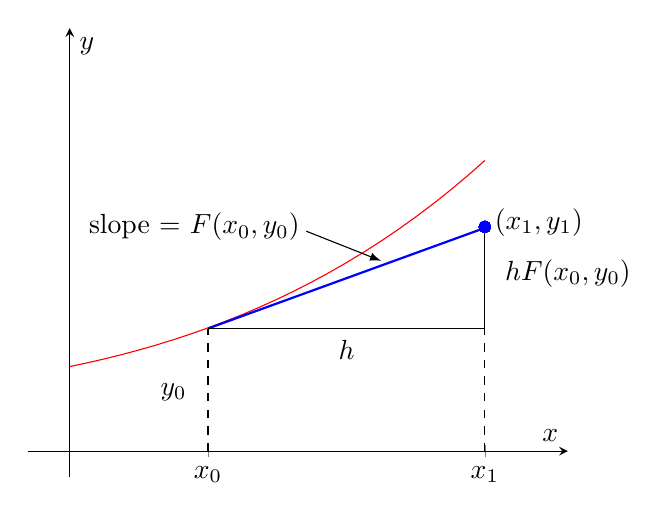
\begin{tikzpicture}
    \begin{axis}[xmin = -0.1, xmax = 1.2, xtick = {0.333, 1}, xticklabels = 
    {$x_0$, $x_1$}, ymin = -0.3, ymax = 5, ytick = \empty, axis lines = center, 
    xlabel = $x$, ylabel = $y$, clip = false]
    \addplot[red, domain = 0:1]{-1*x + 2*e^x - 1};
    \addplot[blue, thick, domain = 0.333:1]{(0.333 + 1.45)*(x - 0.333) + 1.45};
    \draw[black, dashed](0.333, 0) -- (0.333, 1.45);
    \draw[black, dashed] (1, 0) -- (1, 2.651);
    \draw[black] (0.333, 1.45) -- (1, 1.45);
    \draw[black] (1, 1.45) -- (1, 2.651);
    \addplot[mark=*, blue](1, 2.651);
    \node[] at (0.25, 0.7) {$y_0$};
    \node[] at (0.667, 1.2) {$h$};
    \node[] at (1.2, 2.1) {$hF(x_0, y_0)$};
    \node[] at (1.13, 2.7) {$(x_1, y_1)$};
    \node[] at (0.3, 2.65) {slope = $F(x_0, y_0)$};
    \draw[-latex](0.57, 2.6) -- (0.75, 2.25);
    \end{axis}
\end{tikzpicture}
\caption{Visualization of Euler's method}
\label{fig:eulervis}
\end{figure}

Continuing, once we have found $y_1$, we can then define $x_2 = x_1 + h$ and 
$y_2 = y_1 + hF(x_1, y_1)$. And in general, for an initial-value problem when 
$\frac{dy}{dx} = F(x, y)$ and $y(x_0) = y_0$, we can make an approximation 
with step size $h$ where:
$$y_n = y_{n-1} + hF(x_{n-1},y_{n-1})$$
where $n = 1, 2, 3, \cdots$. 

\textbf{Example}: Use Euler's method with a step size of 0.2 to approximate 
the value of $y(1)$ if $\frac{dy}{dx} = 2x + y$ and $y(0) = 1$. 

\textbf{Solution}: We are given $h = 0.2$, $x_0 = 0$, $y_0 = 1$, and $F(x, y) 
= 2x + y$. This means we will need 5 steps to reach $x_{5} = 1$. So, we know 
that:
$$y_1 = 1 + 0.2[2(0) + 1] = 1 + 0.2[1] = 1.2$$
$$y_2 = 1.2 + 0.2[2(0.2) + 1.2] = 1.2 + 0.2(1.6) = 1.52$$
$$y_3 = 1.52 + 0.2[2(0.4) + 1.52] = 1.984$$

We can continue in this manner. The results are shown in the table:
\begin{center}
\begin{tabular}{|c|c|c|c|}\hline
n & $x_n$ & $y_n$ & $F(x_n, y_n)$ \\\hline
0 & 0 & 1 & 1\\\hline
1 & 0.2 & 1.2 & 1.6\\\hline
2 & 0.4 & 1.52 & 2.32\\\hline
3 & 0.6 & 1.984 & 3.184\\\hline
4 & 0.8 & 2.6208 & 4.2208\\\hline
5 & 1 & 3.46496 & --\\\hline
\end{tabular}
\end{center}

Therefore, $y(1) \approx 3.4696$.

\textbf{Example}: This problem was originally presented as a no-calculator, 
multiple-choice question on the 2012 AP Calculus BC exam. Let $y = f(x)$ be 
the solution to $\frac{dy}{dx} = x - y$ with initial condition $f(1) = 3$. 
What is the approximation of $f(2)$ obtained using Euler's method with two 
steps of equal length starting at $x = 1$?

\textbf{Solution}: The question asks that we use Euler's method two steps. The 
step size should be $h = \frac{x_2 - x_0}{2} = \frac{2 - 1}{2} = \frac{1}{2}$. 
Taking $x_0 = 1$ and $y_0 = 3$, we find that:
$$y_1 = y_0 + h \left[x_0 - y_0 \right]$$
$$y_1 = 3 + \frac{1}{2} \left[1 - 3 \right]$$
$$y_1 = 3 + \frac{1}{2} \left[ -2 \right] = 3 - 1 = 2$$

So our intermediate point is $(x_1, y_1) = (\frac{3}{2}, 2)$. Finding $y_2$:
$$y_2 = y_1 + h \left[x_1 - y_1 \right]$$
$$y_2 = 2 + \frac{1}{2} \left[ \frac{3}{2} - 2 \right]$$
$$y_2 = 2 + \frac{1}{2} \left[\frac{-1}{2} \right] = 2 - \frac{1}{4} 
= \frac{7}{4}$$

So the approximate value of $f(2)$ is $\frac{7}{4}$.

\begin{Exercise}[label = eulercircuit]

In the previous chapter on slope fields, we discussed the behavior of inductors in electronic circuits. As you may recall, capacitors also exhibit more complex behavior than regular resistors. Consider a circuit with a resistor and capacitor (see figure below). Let the resistor have resistance R ohms and the capacitor have capacitance C farads. By Kirchhoff's law, we know that:
$$RI + \frac{Q}{C} = V$$
where Q is the charge on each side of the capacitor and $\frac{Q}{C}$ is the voltage drop across the capacitor. Recall that current is the change in charge over time. Therefore, $I = \frac{dQ}{dt}$, and we can write the differential equation:
$$R \frac{dQ}{dt} + \frac{1}{C}Q = V$$
When the switch is first closed, there is no charge (that is, $Q(0) = 0$). If the resistor is $5 \Omega$, the battery is $60 V$, and the capacitor is $0.05 F$, use Euler's method with a step size of 0.1 to estimate the charge after half a second. 

    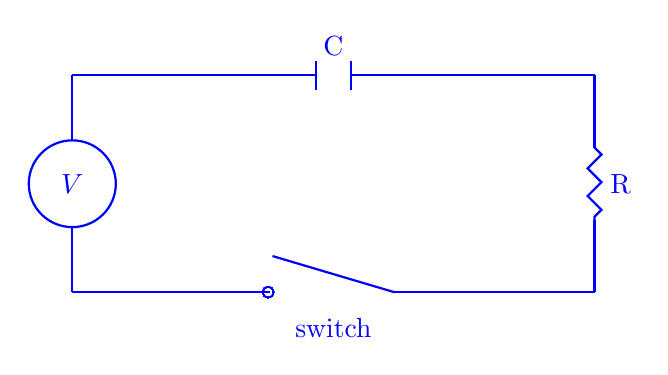
\begin{tikzpicture}
	\begin{axis}[xmin = -3.1, xmax = 3.1, ymin = -3.1, ymax = 3.1, axis lines = 
	none, clip = false]
	\draw[blue, thick](-3, 1.5) -- (-0.2, 1.5);
        \draw[blue, thick] (0.2, 1.5) -- (3, 1.5);
        \draw[blue, thick] (-0.2, 1.3) -- (-0.2, 1.7);
        \draw[blue, thick] (0.2, 1.3) -- (0.2, 1.7);
        \draw[blue, thick](3,1.5) -- (3, 0.5);
        \draw[decorate, decoration = zigzag, color=blue, thick] 
        	(3, 0.5) -- (3, -0.5);
        \draw[blue, thick] (3, -0.5) -- (3, -1.5);
        \draw[blue, thick] (3, -1.5) -- (0.7, -1.5);
        \draw[blue, thick] (0.7, -1.5) -- (-0.7, -1);
        \draw[blue, thick] (-0.73, -1.5) -- (-3, -1.5);
        \addplot[blue, mark=o](-0.75, -1.5);
        \draw[blue, thick] (-3, -1.5) -- (-3, -0.6);
        \draw[blue, thick] (-3, 0.6) -- (-3, 1.5);
        \draw[blue, thick] (-3, 0) ellipse (0.5 and 0.6);
        \node[blue] at (-3, 0) {$V$};
        \node[blue] at (0, -2) {switch};
        \node[blue] at (3.3, 0) {R};
        \node[blue] at (0, 1.9) {C};
        \end{axis}
    \end{tikzpicture}
\end{Exercise}

\begin{Answer}[ref = eulercircuit]
Substituting the given values, we find that $(5)\frac{dQ}{dT} + \frac{1}{0.05}Q = 60$. Solving for $\frac{dQ}{dt}$:
$$(5) \frac{dQ}{dt} + (20)Q = 60$$
$$\frac{dQ}{dt} + 4Q = 12$$
$$\frac{dQ}{dt} = 12 - 4Q$$
We also know that $Q(0) = 0$. Using Euler's method with step size $h = 0.1$, $Q(0.1) \approx Q(0) + h \left[12 - 4Q(0) \right] = 0 + 0.1 \left[12 - 4(0) \right] = 1.2$. And $Q(0.2) \approx Q(0.1) + h \left[12 - 4Q(0.1) \right] = 1.2 + 0.1 \left[12 - 4(1.2) \right] = 1.92$. And $Q(0.3) \approx Q(0.2) + h \left[12 - 4Q(0.2) \right] = 1.92 + 0.1 \left[ 12 - 4(1.92) \right] = 2.352$. And $Q(0.4) \approx Q(0.3) + h \left[12 - 4Q(0.3) \right] = 2.352 + 0.1 \left[ 12 - 4(2.352) \right] = 2.6112$. And finally, $Q(0.5) \approx Q(0.4) + h \left[12 - 4Q(0.4) \right] = 2.6112 + 0.1 \left[12 - 4(2.6112) \right] = 2.76672$. Because we are finding a charge, the unit it Coulombs (C), so our final answer is $Q(0.5) \approx 2.77 C$.
\end{Answer}

\begin{Exercise}[label = euler1]
[This problem was originally presented as a calculator-allowed, free-response 
question on the 2012 AP Calculus BC exam.] The function $f$ is twice-
differentiable for $x > 0$ with $f(1) = 15$ and $f''(1) = 20$. Values of $f'$, 
the derivative of $f$, are given for selected values of $x$ in the table 
below. Use Euler's method, starting at $x = 1$ with two steps of equal size, 
to approximate $f(1.4)$. Show the computations that lead to your answer. 
	\begin{center}
		\begin{tabular}{|c|c|c|c|c|c|}\hline
		$x$ & 1 & 1.1 & 1.2 & 1.3 & 1.4\\\hline
		$f'(x)$ & 8 & 10 & 12 & 13 & 14.5\\\hline
		\end{tabular}
	\end{center}
\end{Exercise} 

\begin{Answer}[ref = euler1]
We are given $x_0 = 1$ and $x_2 = 1.4$. Therefore we will use step size $h = 
\frac{1.4 - 1}{2} = \frac{0.4}{2} = 0.2$. Taking $x_0 = 1$ and $y_0 = f(1) = 
15$, we find $y_1$: $y_1 = y_0 + h \cdot f'(x_0) = 15 + 0.2 \cdot f'(1) = 15 + 
0.2(8) = 15 + 1.6 = 16.6$. And then $y_2 = y_1 + h \cdot f'(x_1) = 16.6 + 0.2 
\cdot f'(1.2) = 16.6 + 0.2(12) = 16.6 + 2.4 = 19$. Therefore, $f(1.4) \approx 
19$. 
\end{Answer}